\section{Broadening the Dark Matter Reach}\label{sec:broaderdarkmatter}

Liquid xenon experiments have already demonstrated that they are versatile detectors with significant sensitivity to a variety of non-WIMP dark matter models. Traditionally, WIMPs are searched-for using analyses that exploit the electronic/nuclear recoil discrimination capability of liquid xenon and achieve the lowest nuclear recoil background of any dark matter direct detection technology. To broaden this reach, a number of different analyses and technologies are available as presented in this section. This in turn enables liquid xenon experiments to achieve competitive sensitivity to a number of dark matter models that are also described here. In particular, subsections~\ref{sec:dpe}--\ref{sec:hydrodoping} describe dedicated analyses and technologies to lower the energy threshold of liquid xenon TPCs. Subsections~\ref{sec:upscattdm}--\ref{sec:bosonicwimp} describe models that especially profit from such lower thresholds, and subsections~\ref{sec:bosonicwimp}--\ref{sec:mirrordm} models where the signal is in the electronic recoil band. Subsections~\ref{sec:maginelasticdm} and~\ref{sec:planck} describe two models that require dedicated analyses to increase the reach of liquid xenon TPCs to complex interactions and up to Planck mass dark matter, respectively.

With the WIMP model being probed extensively by experiment, the community is in parallel starting to work on detector concepts that can probe dark matter over a much wider mass range~\cite{Battaglieri:2017aum}, in particular covering thermal relic particles in the $\n{MeV/c^2}-\n{GeV/c^2}$ mass range~\cite{Essig:2011nj,Essig:2013lka,Hochberg:2014dra,Kuflik:2015isi,Alexander:2016aln,Battaglieri:2017aum}. Searches in this lower mass range were pioneered with liquid xenon detectors~\cite{Essig:2012yx}. While many experiments optimized for very low-energy recoils now exist~\cite{Agnese:2015nto,Angloher:2015ewa,Petricca:2017zdp,Angloher:2017sxg,NEWS-G:2017pxg}, liquid argon~\cite{Agnes:2018ves,Agnes:2018oej} and xenon~\cite{Essig:2017kqs,Akerib:2018hck,Aprile:2019xxb} TPCs still remain the leading technologies even for sub-GeV masses. There is thus significant interest in achieving the lowest-possible energy threshold in a next-generation liquid xenon detector.

\subsection{Double Photoelectron Emission}\label{sec:dpe}

In the traditional analysis where both primary scintillation (S1) and ionization (S2) signals are read out, the energy threshold of two-phase liquid xenon TPCs is set by the smallest scintillation signal that can be confidently discriminated from background sources. Typically, dark matter experiments require an $n$-fold coincidence of PMTs within a short time window for a pulse to be classified as an S1. The optimal value of $n$ (typically in the range 2--4) is a compromise between signal efficiency and the rejection of fake S1 pulses, caused by random coincidences of PMT dark counts~\cite{Aprile:2020thb}.

This methodology makes no attempt to otherwise discriminate dark count background pulses from actual photon-induced pulses. However, it is known that, for some PMT photocathodes, the energy of the liquid xenon scintillation photons (175\,nm or 7\,eV~\cite{Fuji:2015}) is enough to produce two photoelectrons on the PMT photocathode a fraction of the time, resulting in pulses that are on average twice as large as a single photoelectron pulse.

\begin{figure}[!htbp]  
\begin{center}
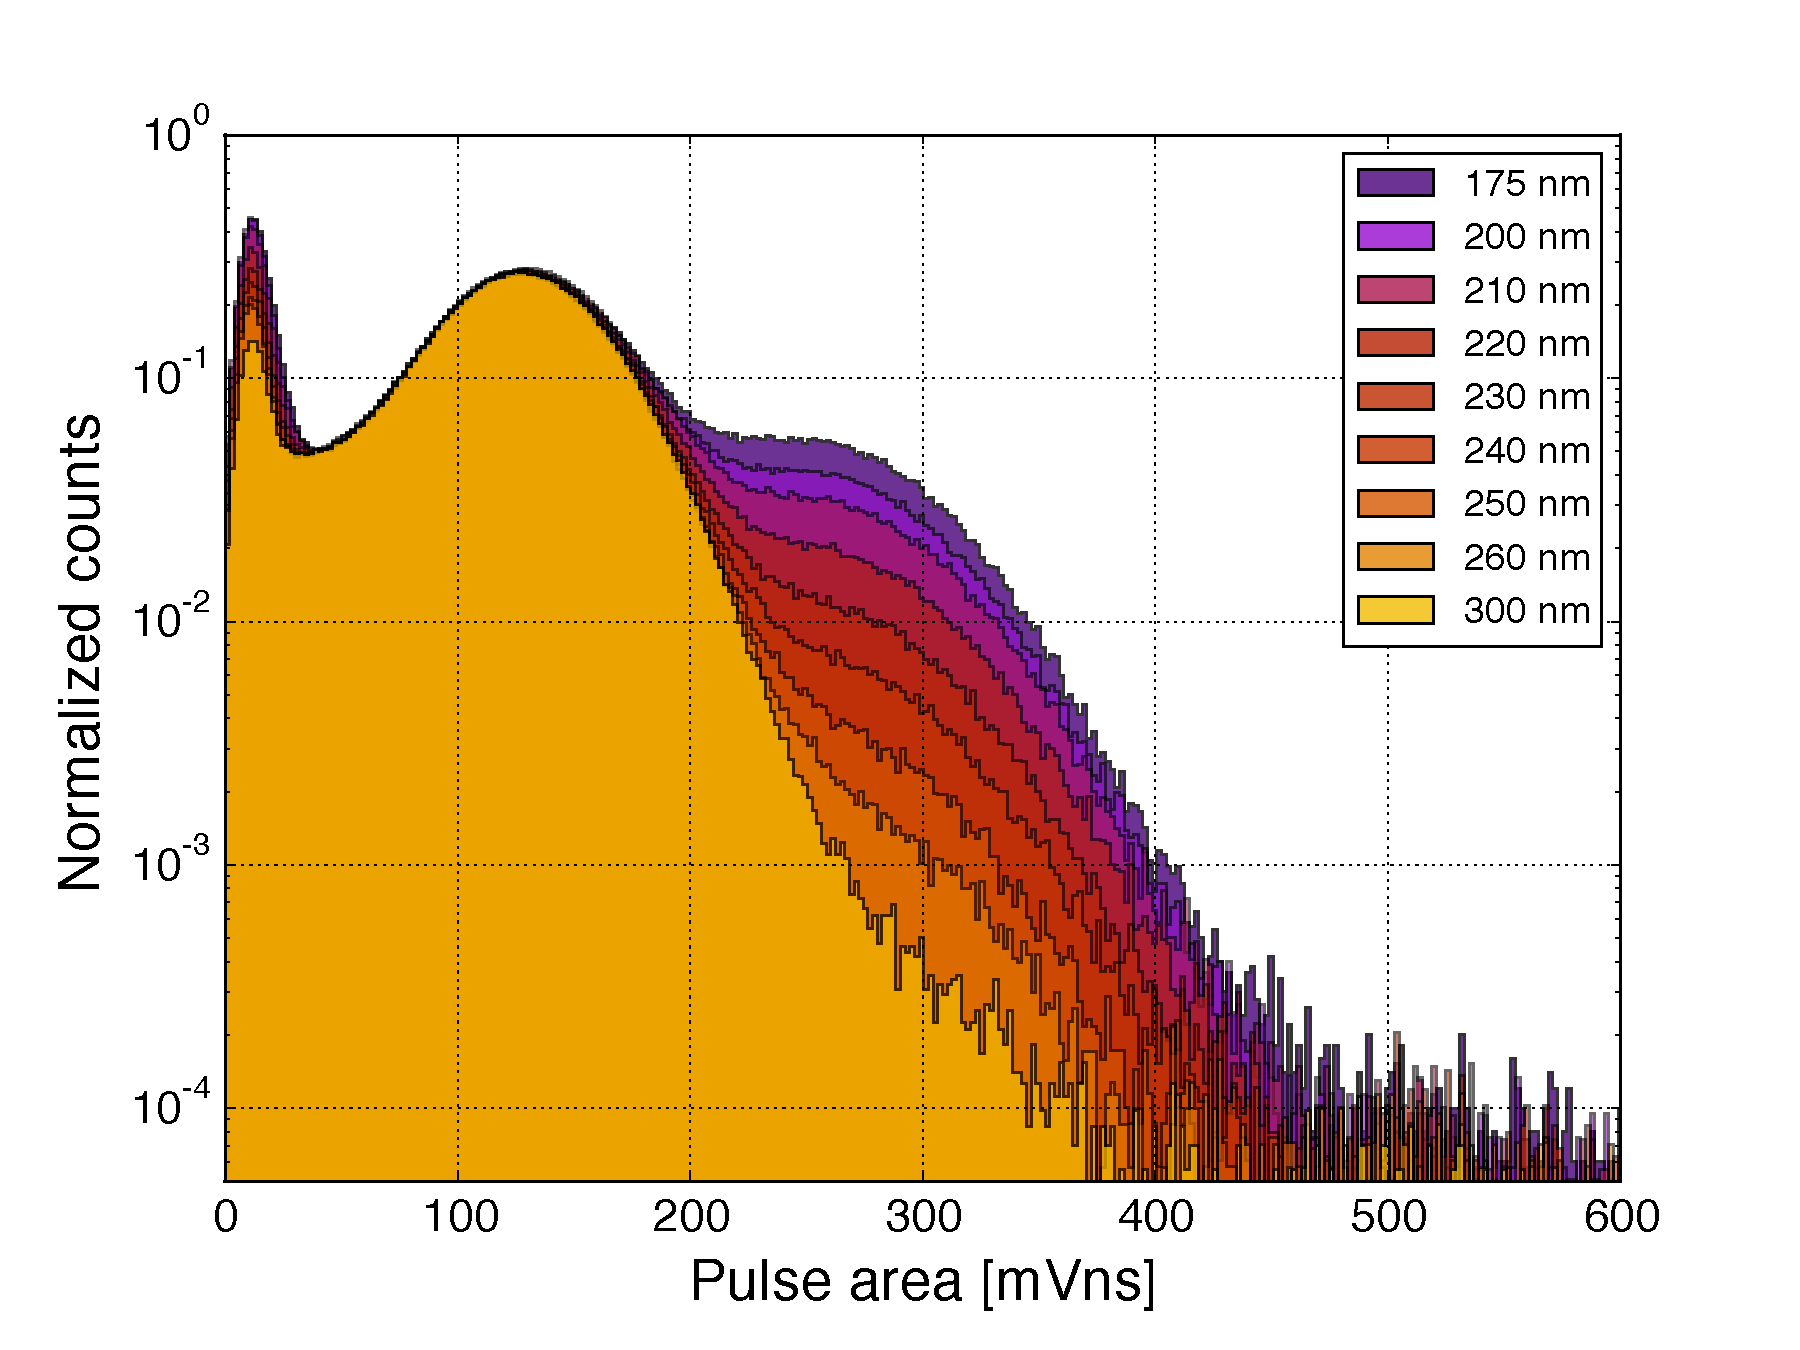
\includegraphics[width=0.99\columnwidth]{fig_R11410_rainbow_plot.pdf}
\caption{Superposition of single photon pulse area spectra of a R11410 PMT for different wavelengths. Each spectrum is normalized by the integral in the region between 50--120~mV~ns in order to show the effect more clearly. Figure from~\cite{Faham:2015kqa}.}
\label{fig:R11410_rainbow_plot}
\end{center} 
\end{figure}

This so-called Double Photoelectron Emission (DPE) effect can therefore be exploited to increase the signal efficiency beyond the standard $n$-fold optimisation, provided that the DPE fraction and efficiency gain can be properly calibrated. This requires the precise determination of the PMT DPE probability, which depends strongly on the wavelength of the impinging light, as well as on the composition and thickness of the photocathode. For the Hamamatsu R11410 PMT model (used e.g.~in XENON1T, XENONnT, RED, and LZ), a wavelength scan was performed with single photons down to the VUV range on one unit~\cite{Faham:2015kqa} (see \autoref{fig:R11410_rainbow_plot}). The inter-PMT variability due to the photocathode manufacturing process has also been measured at low temperature with a batch of 35 R11410-22 PMTs~\cite{Paredes:2018hxp}. Measuring the DPE probability is also crucial for pulse area calibration. A pulse area in `photoelectrons' does not represent the number of photon hits detected, but can be understood and calibrated if the DPE probability is known. Experiments have reported average values of their PMT DPE probability of around $\sim$10--20\% given liquid xenon scintillation light~\cite{Araujo:2020rwg, Akerib:2019zrt}.

\begin{figure}[!htbp]  
\begin{center}
\includegraphics[width=0.99\columnwidth]{fig_LUX_DPE_limits.eps}
\caption{90\%~CL upper limits on the spin-independent WIMP-nucleon cross section obtained using the single-photon population producing Double Photoelectron Emission in the LUX 2013 WIMP search. The observed limit with a 0.3~keV NR energy cut-off is shown in solid black, with 1$\sigma$ and 2$\sigma$ sensitivity bands shown in green and yellow. The dashed black line is derived from the same analysis but with a model cut-off at 1.1~keV. Both of these results correspond to the NEST v.2.0.0 model. The upper limit using a 0.3~keV NR energy cut-off with the newer NEST v.2.0.1 model is shown using a dotted black line. Also shown are other results current at the time, namely from the LUX 2013 search~\cite{Akerib:2015rjg} (gray), the LUX complete exposure~\cite{Akerib:2016vxi} (red), DarkSide-50~\cite{Agnes:2018ves} (green), PandaX-II~\cite{Cui:2017nnn} (blue), PICO60~\cite{Amole:2017dex} (lilac) and CDMSLite~\cite{Agnese:2015nto} (purple). Figure from~\cite{Akerib:2019zrt}.}
\label{fig:lux_DPE_limits}
\end{center} 
\end{figure}

The LUX experiment exploited this DPE to lower the coincidence condition from two PMTs to just a single PMT with an S1 pulse consistent with DPE~\cite{Akerib:2019zrt} (\autoref{fig:lux_DPE_limits}). In general, an experiment may lower its $n$-fold condition by requiring that a subset of PMT hits are consistent with DPE. A PMT with a low dark count rate and high DPE probability might enhance the low-energy reach of a next-generation dark matter experiment with a straightforward extension of the analysis~\cite{Akerib:2021pfd}.

\subsection{Charge-Only Analysis}\label{sec:s2only}

Interactions from WIMP candidates below $\sim\n{GeV/c^2}$ would produce scintillation (S1) signals close to or below the typical low-energy threshold of liquid xenon TPCs. This loss of efficiency can be bypassed by removing the requirement that the S1 signal be detected at all, and leveraging the inherent gain in the S2 signal~\cite{Aprile:2016wwo, Agnes:2018ves, Aprile:2019xxb, Akerib:2021pfd}. Relaxing the requirement of an observed S1 allows events which resulted in even a single extracted electron to be analyzed. This increased sensitivity to low-mass dark matter candidates comes at the expense of particle discrimination (usually from the S2/S1 ratio) and accurate determination of the z-coordinate (usually from the delay between the S1 and S2 signals). While sometimes these analyses still make use of S1 pulses to reject background events, when they do not require an S1 to be present, they are commonly referred to as `charge-only' or `S2-only' analyses.

Thus far, charge-only analyses have been background-limited due to large single- and few-electron backgrounds, which have yet to be reliably quantified and mitigated~\cite{Akerib:2020jud, Kopec:2021ccm, Bodnia:2021flk, Akimov:2016rbs, Aprile:2013blg, Sorensen:2017kpl, Sorensen:2017ymt}. The extended drift volume of a next-generation detector may be subject to stronger electron lifetime effects, but will also provide improved identification of S2s originating from the bottom of the detector because of increased electron diffusion (resulting in wider S2 pulses). Additionally, xenon contamination from out-gassing or surface detachment of impurities will benefit from the relative scaling of volume and surface area. Despite being background limited, charge-only analyses have been used to set leading limits on dark matter interaction rates, see \autoref{fig:sub_GeV}. The sensitivity of liquid xenon TPCs to signals at the level of single electrons results in leading sensitivity to sub-GeV WIMPs as well as other particle models. A charge-only analysis in a next-generation detector will further improve this sensitivity over the current generation of xenon TPCs. 

\begin{figure}[!htbp] 
\begin{center}
\includegraphics[width=0.99\columnwidth]{fig_x1t_subGeV.pdf}
\caption{The 90\% confidence level upper limits (black lines with gray shading above) on spin-independent dark matter-nucleus scattering with the dark matter mass, $m_\chi$, on the horizontal axis. The thick black line is the result from the XENON1T charge-only analysis. Other results from XENON1T in blue~\cite{Aprile:2018dbl}, LUX in orange~\cite{Akerib:2016vxi}, PandaX-II in magenta~\cite{Ren:2018gyx}, DarkSide-50 in green~\cite{Agnes:2018ves}, XENON100 in turquoise~\cite{Aprile:2016wwo, Aprile:2016swn}. Dotted lines show the XENON1T limit when assuming the $Q_y$ from NEST v2.0.1~\cite{szydagis_m_2019_3357973} cut off below 0.3~keV. The limits exhibit a steep change at 17.5~GeV$/c^2$ because the observed count changes from 10 to 3 events in the ROIs left and right of this change, respectively. Figure taken from~\cite{Aprile:2019xxb}.}
\label{fig:sub_GeV}
\end{center} 
\end{figure}

\subsection{General Dark Matter-Induced Atomic Responses}\label{sec:genatomresp}

A dark matter particle with mass in the MeV--GeV range can deposit enough energy in the collision with an electron in a xenon atom to ionise the target and produce a detectable S2 signal in a TPC detector~\cite{Kopp:2009et,Essig:2011nj}. This charge-only analysis has mainly been performed with models where the interaction between dark matter and electrons is mediated by a new hypothetical force carrier such as the dark photon~\cite{Agnes:2018oej,Aprile:2019xxb}. To avoid confusion, here the dark photon acts as force carrier, as opposed to the analysis described in \autoref{sec:dark_photon}, where the dark photon itself is the dark matter candidate. In this framework, the total ionisation rate for a given xenon orbital can be expressed in terms of a single target-dependent ionisation form factor, which is a function of the initial and final state electron wave functions~\cite{Kopp:2009et,Essig:2011nj}.

Xenon detectors can also probe more complex models, such as those where the amplitude for dark matter scattering by a free electron, $\mathcal{M}$, depends on the initial electron momentum~\cite{Catena:2019gfa}. These include models where dark matter couples to electrons via magnetic dipole or anapole interactions. By expanding $\mathcal{M}$ using effective theory methods similar to the ones previously discussed in the context of dark matter-nucleon interactions (see \autoref{sec:nreft}), Reference~\cite{Catena:2019gfa} found that the most general form for the total ionisation rate of a given xenon orbital is a linear combination of four target-dependent atomic responses, which are defined in terms of initial and final state electron wave function overlap integrals. Assuming that dark matter is made of fermions with mass in the MeV-GeV range and interactions dominated by electromagnetic moments of higher order, such as the electric and magnetic dipoles or the anapole moment, reference~\cite{Catena:2020tbv} showed that liquid xenon TPCs can shed light on whether dark matter is a Dirac or Majorana particle. By using Monte Carlo simulations and a non-trivial extension of the likelihood ratio test to the case where one of the hypotheses lies on the boundary of the parameter space, only about $45-610$ signal events are required to reject Majorana dark matter in favour of Dirac dark matter at 3~sigma confidence level. 

\subsection{Migdal Effect and Bremsstrahlung}\label{sec:migdal}

\begin{figure}[!htbp] 
\begin{center}
\includegraphics[width=0.99\columnwidth]{fig_x1t_migdal.pdf}
\caption{Limits on the spin-independent light mediator dark matter-nucleon interaction cross section at 90\% confidence level using signal models from the Migdal effect and Bremsstrahlung in the XENON1T experiment with the S1-S2 data (blue contours and lines) and charge-only data (black contours and lines). The solid and dashed (dotted) lines represent the lower boundaries (also referred to as upper limits) and Midgal (Bremsstrahlung) upper boundaries of the excluded parameter regions. Green and yellow shaded regions give the 1 and 2$\sigma$ sensitivity contours for upper limits derived using the S1-S2 data, respectively. The upper limits on the spin-independent dark matter-nucleon interaction cross sections from LUX~\cite{Akerib:2018hck} and XENON1T charge-only (elastic nuclear recoil results)~\cite{Aprile:2019xxb} are also shown. Figure taken from~\cite{Aprile:2019jmx}.}
\label{fig:migdal}
\end{center} 
\end{figure}

\begin{figure}[!htbp]
    \includegraphics[width=0.99\columnwidth]{fig_migdal_s2o_projection.pdf}
    \caption{Spin-independent sensitivity for the electronic recoil-inducing Migdal effect for the case of a heavy scalar mediator. The S1-S2 sensitivity (black, solid) and the charge-only sensitivity (violet, solid) are shown. The charge-only analysis improves the sensitivity by more than two orders of magnitude with respect to the standard S1-S2 analysis (red, solid). Experimental limits from similar analyses in LUX (blue, solid)~\cite{Akerib:2018hck}, XENON1T (green, solid)~\cite{Aprile:2019xxb} and CDEX (gray, solid)~\cite{Liu:2019kzq} are also shown.\label{fig:migdalProjection}}
\end{figure}

The progressive loss of the scintillation (S1) response with decreasing nuclear recoil energy impede the ability of liquid xenon TPCs to reach sensitivity for sub-GeV dark matter masses. However, the standard dark matter-nucleus interaction can also induce an inelastic atomic scattering signal. 
The Migdal effect~\cite{Migdal:1941} predicts the ionization of the atom with some (small) probability due to the sudden nuclear acceleration caused by the dark matter collision, resulting in excitation and ionization processes from the electrons~\cite{Ibe:2017yqa}. Since electronic recoils produce a more detectable signal than nuclear recoils, this channel enables liquid xenon detectors to reach dark matter masses of $\mathcal{O}(100\ {\textrm{MeV}/c^2})$~\cite{Dolan:2017xbu,Akerib:2018hck,Aprile:2019jmx}, see \autoref{fig:migdal}. The sensitivity of liquid xenon detectors to sub-GeV dark matter achieved using the Migdal effect is competitive with other detectors that are dedicated to searches of light dark matter~\cite{NEWS-G:2017pxg,CRESST:2019jnq,SuperCDMS:2020ymb}. \autoref{fig:migdalProjection} shows a conservative projected Migdal sensitivity for a next-generation detector assuming LZ detector parameters with an extended exposure of 300~tonne-years, equivalent to e.g.~a 56~tonne fiducial mass and 5.4~live-years. 

Similar to the Migdal effect, nuclear Bremsstrahlung searches leverage the fact that in liquid xenon at low energies, electronic recoils produce a stronger signal than nuclear recoils~\cite{Kouvaris:2016afs}. Bremsstrahlung searches consider the emission of a photon from the recoiling atomic nucleus. In the atomic picture this can be viewed as the dipole emission of a photon from a xenon atom that has been polarized in the dark matter-nucleus scattering. In xenon, the emission of the Bremsstrahlung photon is more heavily suppressed compared to the Migdal effect and hence results in a weaker signal. The theoretical motivation and event rates for Bremsstrahlung have been derived in~\cite{Kouvaris:2016afs} and searches using liquid xenon detectors have been published in~\cite{Akerib:2018hck,Kobayashi:2018jky,McCabe:2017rln}.

\subsection{Hydrogen Doping}\label{sec:hydrodoping}

Kinematically, the large xenon nucleus (average mass 122~GeV) is not well suited for an efficient transfer of energy from Galactic dark matter with mass $\lesssim$1~GeV/$c^2$. As a result, nearly all of the resulting xenon nuclear recoils fall below the energy threshold for detection. A possible solution for enhancing the sub-GeV sensitivity of liquid xenon TPCs is to dissolve a lighter species in the liquid xenon bulk~\cite{Akerib:2021hydrox}. In this configuration, the lighter nucleus becomes the dark matter target, and the xenon becomes the sensing medium.

This strategy exploits two of the primary advantages of the liquid xenon medium. First, the high atomic number and density of liquid xenon provides excellent self-shielding of external backgrounds from the central volume of the detector. Such a suppression would not be possible in a similarly-sized detector comprised of the light species alone. Second, the high yield of detectable quanta (electrons and photons) resulting from low-energy particle interactions makes xenon an ideal sensor for the recoiling light nuclei.

Having the lightest nucleus of any element, hydrogen is kinematically the best candidate species for detecting sub-GeV dark matter interactions. The lone proton comprising hydrogen's nucleus additionally provides unique sensitivity to the spin-dependent dark matter coupling to protons. Likewise, doping the xenon target with deuterium would provide similar sensitivity to the neutron-only couplings. Helium is also a viable option as the light mass target species, but its spin-dependent sensitivity would be comparatively poor. Introduction of helium into the detector might not be suitable if PMTs are used as a photosensor due to its ability to diffuse into and degrade the PMT vacuum. However, helium could be considered as a dopant if silicon photomultipliers (SiPMs) are used to detect light signals instead of PMTs.

\subsection{Upscattered Dark Matter}\label{sec:upscattdm}

The sensitivity reach of liquid xenon detectors for sub-GeV dark matter is significantly enhanced if some dark matter particles receive a kinematic boost from up-scattering with cosmic rays~\cite{Bringmann:2018cvk,Alvey:2019zaa,Cappiello:2019qsw,Dent:2019krz,Bondarenko:2019vrb,Wang:2019jtk}. This process, often denoted CRDM, will create a small population of fast or even relativistic dark matter particles. This in turn provides sensitivity to liquid xenon experiments to dark matter with masses several orders of magnitude below 1~GeV. Cosmic ray up-scattered dark matter is only a fraction of the Galactic dark matter population, with an abundance and flux that depends on the dark matter-cosmic ray scattering cross section, the local dark matter density, and the local interstellar spectrum of cosmic rays. Relatively large cross section values of e.g. $\sigma_{\chi N}\gtrsim 10^{-31}{\rm{cm}}^2$ for $m_\chi = 1$~GeV are required to have a notable impact on the sensitivity of a typical liquid xenon detector. For spin-independent interactions, liquid xenon experiments are competitive with and complementary to existing neutrino experiments~\cite{Bringmann:2018cvk, Cappiello:2019qsw,  PROSPECT:2021awi}, which have sensitivity in a similar region of parameter space.

Another upscattering mechanism extending the sensitivity of liquid xenon detectors to dark matter masses down to keV scales is a process called ``solar reflection''~\cite{An:2017ojc,Emken:2017hnp}. This is based on the observation that scatterings on thermal electrons and nuclei within the Sun can accelerate light dark matter particles. This could give rise to an observable flux of highly energetic particles in a liquid xenon TPC detector.

\subsection{Dark Matter Annihilation Products}\label{sec:dmproducts}

In several models of so-called ``neutrino portal" dark matter, Galactic dark matter self-annihilates into neutrinos~\cite{Cherry:2014xra,GonzalezMacias:2015xbi,Becker:2018rve,Lamprea:2019qet,Patel:2019zky}. These in turn may be detected at direct detection experiments with high rates via coherent elastic neutrino-nucleus scattering (see \autoref{sec:cevns}). A next-generation liquid xenon detector would be sensitive to the flux of these neutrinos for dark matter mass (respective neutrino energy) of $[0.01-1]\1{GeV/c^2}$~\cite{McKeen:2018pbb}. The sensitivity to this neutrino flux would complement neutrino detectors such as Super-Kamiokande. Similarly, dark matter that annihilates to a second component of nucleophilic, ``boosted" dark matter could also be discovered. A next-generation liquid xenon TPC will be sensitive to the effective baryonic coupling of thermal boosted dark matter that is as low as the weak interaction~\cite{McKeen:2018pbb}.

Alternatively, dark matter may annihilate or decay within the target volume of future liquid xenon detectors~\cite{Undagoitia:2021tza}. Considering deposited energies up to a few MeV, the relevant final states include annihilation into $\gamma\gamma$ and $e^-e^+$, and decays into $\gamma\gamma$, $\gamma\nu$ and $e^-e^+$. Although the sensitivity obtained is not as high as the current limits from cosmological considerations~\cite{Slatyer:2015jla} and X-ray measurements~\cite{Ng:2019gch}, this is a complementary approach in a well-understood background environment and free of the large uncertainties typically present in indirect detection experiments.

\subsection{Bosonic Super-WIMPs}\label{sec:bosonicwimp}

Super Weakly Interacting Massive Particles, or super-WIMPs, make up a broad class of dark matter candidates that couple to Standard Model particles with cross sections far smaller than the weak scale~\cite{Feng:2003xh}. These include fermions such as sterile neutrinos~\cite{Dodelson:1993je} and gravitinos, both of which only couple to the Standard Model gravitationally and thus are impossible to observe in a typical direct detection experiment. However, keV-scale bosonic super-WIMPs can couple to light Standard Model particles in such way to be observed with low-background experiments~\cite{Pospelov:2008jk}. Here we give two examples of super-WIMPs, dark photons and axion-like particles, and discuss related signals.

\subsubsection{Dark Photons}\label{sec:dark_photon}

Dark photons are vector bosonic super-WIMPs. Proposed as a force carrier for a dark sector, they can also serve as a dark matter candidate if they are stable enough~\cite{Pospelov:2008jk}. The dark photon kinetically mixes with the SM photon, and can be absorbed in a detector medium with a cross section proportional to the photoelectric cross section. The expected signal is therefore a mono-energetic electronic recoil peak at the dark photon mass. Direct detection experiments have set competitive constraints on kinetic mixing parameter $\kappa$ of dark photons, in a mass range from several to hundreds of keV~\cite{An:2014twa}. A next-generation detector such as the one discussed here will have improved sensitivity to this mixing parameter $\kappa$. Further, dedicated low-energy calibrations, for example using $^{37}$Ar diluted in the liquid xenon, will help to improve the search in the keV mass range and reduce the relevant detector-specific systematics to negligible levels for a discovery experiment. Using a low-energy charge-only analysis (\autoref{sec:s2only}), the sensitive mass range can be extended to the sub-keV level.

\subsubsection{Axions and Axion-Like Particles}

The axion is a pseudoscalar Goldstone boson originally proposed as a solution to the strong CP problem of QCD~\cite{PecceiQuinn_1977,Weinberg:1977ma,Wilczek:1977pj}. Stable and massive, axions are also well-motivated dark matter candidates~\cite{Preskill:1982cy,Abbott:1982af,Dine:1982ah}. They couple to the Standard Model very weakly, with couplings suppressed by a high energy scale $f_a$. QCD axions -- i.e. axions that also solve the strong CP problem -- have couplings $g \sim 1/f_a$ that are proportional to the axion mass $m_a$ which is constrained to be $m_a \lesssim 1\1{eV/c^2}$ by astrophysical bounds~\cite{Raffelt:2006cw,Sikivie:2006ni,Ayala:2014pea,Chang:2018rso,Capozzi:2020cbu} and the solar axion helioscope CAST~\cite{Anastassopoulos:2017ftl}. Such axions are below the sensitivity reach of detectors like the one discussed here, and require dedicated experiments. However, axions produced in the Sun would have thermal spectra with keV energies, and could be detected with a xenon TPC as discussed in \autoref{sec:solar_axions}.

Axion-like particles (ALPs) are the phenomenological generalization of the QCD axion in that they share the same properties, but the strict relationship between the mass and the scale $f_a$ is relaxed. These particles do not solve the strong CP problem, but nevertheless are good dark matter candidates and can show up abundantly in theories for physics beyond the standard model, in particular string theory~\cite{Witten:1983ar,Conlon:2006tq,Arvanitaki:2009fg,Arvanitaki:2010sy,Cicoli:2012sz, Arvanitaki:2014wva}. In a similar way to dark photons, ALPs can be detected via an analogous process to the photoelectric effect~\cite{Derevianko:2010kz}. For dark matter ALPs, the resulting signal is again a mono-energetic spectrum of electronic recoils at the ALP mass, with an event rate proportional to the square of the dimensionless axion-electron coupling~$g_{ae}$. 

Due to their ultra-low electronic recoil background levels, liquid xenon TPCs have placed the strongest constraints to date on keV ALP dark matter~\cite{Aprile:2014eoa, Abe:2014zcd,Akerib:2017uem, Fu:2017lfc,Abe:2018owy,Aprile:2019xxb,Aprile:2020tmw,Zhou:2020bvf}, and next generation detectors will likely continue to set world-leading constraints~\cite{Aalbers:2016jon}.

\subsubsection{Solar Axions, Dark Matter, and Baryon Asymmetry}

As discussed in \autoref{sec:solar_axions}, a liquid xenon TPC can detect the QCD axion and axion-like particles from the Sun for sufficiently large couplings of the axion with electrons or photons. Such relatively large couplings correspond to a small decay constant of the axion. In this case, the cosmological abundance of axions produced by conventional mechanisms~\cite{Abbott:1982af,Dine:1982ah,Preskill:1982cy,Davis:1986xc} is too small for the axion to explain the observed dark matter. However, the axion abundance can be large enough to be dark matter in the various scenarios proposed in~\cite{Sikivie:1982qv,Visinelli:2009kt,Hiramatsu:2010yn,Co:2017mop,Co:2018mho,Co:2019jts,Hook:2019hdk}, with couplings that are sufficiently large to be detected in the proposed detector. 

In one such cosmological scenario for example~\cite{Co:2019jts}, a non-zero field velocity delays the onset of field oscillations, enhancing the axion abundance relative to the conventional misalignment mechanism. For axion-like particles, this field velocity can simultaneously explain the baryon asymmetry of the universe~\cite{Co:2020xlh}. Fitting the ratio of dark matter to baryon abundances predicts the axion coupling in terms of its mass $m_a$
\begin{equation}
g_{a \gamma} \simeq 2\times 10^{-11}c_\gamma~{\rm GeV}^{-1} \left(\frac{m_a}{\rm meV}\right)^{1/2},
\end{equation}
where $c_\gamma$ is a model-dependent constant of order unity. For any axion mass, this is much larger than the photon coupling of the QCD axion. A next-generation liquid xenon TPC with a 1000 ton-year exposure can probe this coupling down to $g_{a\gamma}\sim 3 \times 10^{-11} {\rm GeV}^{-1}$~\cite{Dent:2020jhf}, corresponding to $m_a \sim$~meV.

\subsection{Luminous Dark Matter}\label{sec:lumidm}

It is possible to construct models where the dominant signal of the dark matter originates from photons. These photons could be observed in direct detection experiments as a monoenergetic line produced by dark matter decay from an excited state~\cite{Feldstein:2010su,Pospelov:2013nea}. The excited state could be populated through upscattering in or near the detector (and have short lifetimes $\sim1\,\mu s$) or in the Earth (lifetimes $\sim(1-10)$\,s). For this scenario to work, the elastic cross section needs to be small relative to the inelastic cross section. A simple way to achieve this is with a magnetic dipole operator which couples two distinct Majorana fermions that have a small, $\mathcal{O}$(keV) mass splitting. Such "Luminous dark matter" was first proposed as a potential explanation of the DAMA/LIBRA modulation~\cite{Feldstein:2010su} and has since been used to explain the recent XENON1T excess~\cite{Bell:2020bes}. While the former scenario is now strongly constrained, the latter scenario will be confirmed or ruled out by a next-generation liquid xenon experiment.

\subsection{Mirror Dark Matter}\label{sec:mirrordm} % both ER and NR

Mirror Dark Matter~\cite{Foot:2007nn} represents the intriguing idea that an exact copy of the Standard Model in the dark sector is invoked with an unbroken symmetry between the two. Mirror dark matter can generate signatures both in nuclear recoils similar to those expected from $\sim 7\1{GeV}/c^2$ WIMPs with a cross section around $10^{-44}\1{cm^2}$, as well as in electronic recoils~\cite{Foot:2010hu,Foot:2014mia,Foot:2018jpo}. Mirror dark matter as a hypothesis is potentially entirely falsifiable by a next-generation liquid xenon experiment~\cite{Clarke:2016eac}.

\subsection{Magnetic Inelastic Dark Matter}\label{sec:maginelasticdm}

A natural scenario where dark matter dominantly scatters off nuclei through an inelastic transition in the dark sector (\autoref{sec:inelasticdarkmatter}) is the case of a magnetic dipole interaction~\cite{Chang:2010en}. This model relies on the fact that fermionic dipole operators vanish for Majorana fermions. Thus, if a dark matter Dirac fermion state is split into two nearly degenerate Majorana fermions, an elastic dipole transition is forbidden, leaving the leading dark matter interaction to be an inelastic magnetic dipole transition. Many examples of dark matter models that can realize this scenario have been studied, see e.g.~\cite{Kumar:2011iy,Patra:2011aa,Weiner:2012gm, Pierce:2014spa}.   

For magnetic inelastic dark matter, the sensitivity of a direct detection experiment is modified by both the kinematic constraints of inelastic transitions and by the dependence on the charge and magnetic dipole moment of the target nuclei~\cite{Chang:2010en}. Depending on the dark matter mass splitting and the size of the dipole moment, the excited dark matter state can also decay in the detector, thus yielding both a nuclear recoil from the initial scatter and an electronic recoil from the decay shortly thereafter. Searching for the photons produced by this decay can be an additional handle on uncovering such a scenario~\cite{Lin:2010sb, Pospelov:2013nea}. A dedicated search has been performed by XENON100~\cite{Aprile:2017kek}, with the proposed experiment providing significantly improved sensitivity not only due to the lower background and longer exposure, but also due to the larger size of the detector which translates into a sensitivity to longer decay times.

\subsection{Dark Matter around the Planck Mass} \label{sec:planck}

\begin{figure}[!htbp]  
\begin{center}
\includegraphics[width=0.99\columnwidth]{fig_multiscatter_SI.pdf}
\caption{Per-nucleon spin-independent scattering cross sections and dark matter masses that can be probed by liquid xenon dark matter detectors via dedicated searches for multi-scatter signals. For cross sections above $\sigma_{\rm MIMP}$ (horizontal green lines) one expects dark matter to scatter multiple times in the detector while transiting. The maximum mass reachable (vertical green lines) is limited by the total integrated flux of dark matter in the detector over the run-time of the experiment. Masses up to and beyond the Planck mass $\simeq 10^{19}\1{GeV/c^2}$ may be probed with a next-generation detector. Figure taken from~\cite{Bramante:2018qbc}.}
\label{fig:multiscatter_SI}
\end{center} 
\end{figure}

The observed local dark matter mass density could be made up of few but very massive dark matter particles with masses around the Planck mass $\simeq 10^{19}\1{GeV/c^2}$, as opposed to numerous lighter particles. Super-massive species are motivated by supersymmetric and grand unified theories~\cite{Kolb:2017jvz}, and their detection could help determine parameters of the early universe such as inflation~\cite{Chung:1998zb}. Their existence could also imply new light mediators beyond the Standard Model~\cite{Davoudiasl:2018wxz}. 

Due to the small number density, the flux of these particles through a given detector would be very low, and thus any detection would both imply and require a very high scattering cross section, such that almost all particles impinging on the detector prompt a signal. When the cross section becomes high enough that these particles would interact more than once in the detector, discovery requires a dedicated analysis looking for multiple-scatter events. Such events are typically discarded in WIMP-like dark matter analyses, leaving many orders of magnitude of unexplored parameter space, see \autoref{fig:multiscatter_SI}. In this multiple scattering regime, a next-generation liquid xenon experiment would be capable of probing dark matter masses up to and beyond the Planck mass $\simeq 10^{19}$~GeV~\cite{Bramante:2018qbc}, in a complementary way to the range that could be probed using dedicated neutrino experiments~\cite{Bramante:2018tos,Clark:2020mna}.
Clusters of dark matter formed through self-attraction~\cite{Butcher:2016hic}, such as ``dark blobs''~\cite{Grabowska:2018lnd} or ``dark nuggets''\cite{Coskuner:2018are} would also be visible as tracks in the detectors.


